Dieses Kapitel gibt einen Überblick über verwendete Technologien und Konzepte.
Zunächst werden relevante Protokolle und deren Funktionsweise erläutert.
Anschließend wird eine Einführung über Kubernetes gegeben.
Die in diesem Kapitel vorgestellten Technologien und Konzepte sind Teil meiner täglichen Arbeit als Software Ingenieur im Bereich der Cloud Nativen Software Entwicklung.

\subsection{Hypertext Transfer Protocol}\label{subsec:hyper-text-transfer-protocol}

Das Hypertext Transfer Protocol (HTTP) ist ein Protokoll zur Kommunikation über das World Wide Web, welches von der Internetengineering Task Force (IETF) standardisiert und weiterentwickelt wird.
Da HTTP sich im OSI-Modell der Anwendungsschicht (Layer 7) zuordnen lässt~\cite{kumar2014osi}, bringt das Protokoll unter anderem die Vorteile mit sich, dass es unabhängig von der darunterliegenden Netzwerktechnologie und einfach erweiterbar ist.
So bildet HTTP die Grundlage für viele weitere Protokolle wie zum Beispiel Hypertext Transfer Protocol Secure (HTTPS)~\cite{rfc2818} zur verschlüsselten Übertragung von Daten oder das Simple Object Access Protocol (SOAP)~\cite{SOAP-20000508} zur Kommunikation zwischen verteilten Systemen.
Aufgrund seiner Erweiterbarkeit und einiger Performanz Optimierungen in der Vergangenheit liegt HTTP heute in den Versionen 1.0, 1.1 und 2 vor.
Eine Version 3 ist momentan in Entwicklung.
In Version 3 ist geplant, von TCP auf das User Datagram Protocol (UDP) in Kombination mit dem Quick UDP Internet Connections (QUICK) Protokoll~\cite{rfc9000} zu wechseln, um die Geschwindigkeit im Netz weiter zu verbessern und HTTP/2 abzulösen~\cite{rfc9114}.
Die folgenden Abschnitte geben einen Überblick über für die folgende Arbeit relevante, versionsspezifische Besonderheiten.

\subsubsection{HTTP/1.0 und HTTP/1.1}
HTTP ist ein textbasiertes, zustandsloses Protokoll, was bedeutet, dass sogenannte aus Klartext bestehende Anfragen (Requests) unabhängig voneinander sind.
Dieser Umstand erlaubt die horizontale Skalierung von Webservern und vereinfacht deren Implementierung.
RFC1945~\cite{rfc1945} spezifiziert HTTP/1.0.
Zur Spezifikation gehört die Definition von Unique Resource Identifiers (URIs), welche gemeinhin bekannt sind als Internetadresse.
Des Weiteren erfolgt die Definition verschiedener HTTP-Methoden wie unter anderen \textit{GET} (Informationsabfrage), \textit{HEAD} (Metadatenabfrage) und \textit{POST} (Hochladen von Informationen) und Status Codes zur Auswertung der Server Antwort (Response).
Nach HTTP/1.0 wird für jeden Request eine neue TCP-Verbindung~\footnote{TCP: Verlustbehaftetes Protokoll zur Übertragung binärer Daten über das Netzwerk.} etabliert, welche nach Übertragung der Antwort wieder geschlossen wird.

Da mit HTTP/1.0 die Grundlagen zur Kommunikation im Web gelegt sind, wird das Protokoll in RFC2616~\cite{rfc2616} um Version HTTP/1.1 erweitert.
Im Wesentlichen werden mit der neuen Version die folgenden Punkte zur Verbesserung der Performanz eingeführt:

\begin{itemize}
    \item \textbf{Persistente Verbindungen:} TCP Verbindungen, welche zwischen Client und Server aufgebaut werden, werden wiederverwendet, anstatt geschlossen zu werden.
    Diese Konfiguration wird in HTTP/1.1 zum Standard, reduziert den Overhead des TCP-Handlings und führt zu schnelleren Antwortzeiten.
    \item \textbf{Pipelining:} Persistente Verbindungen erlauben das Senden mehrerer paralleler Requests, ohne auf die Antwort des Servers zu warten.
    \item \textbf{Chunked Transfer-Encoding:} Daten können in mehreren Teilen übertragen werden.
    Dieses Verhalten erlaubt das Streaming von Daten.
\end{itemize}

\subsubsection{HTTP/2}

Obwohl HTTP/1.1 mit dem Pipelining bereits die parallele Übertragung von Requests ermöglicht, birgt diese Technologie einige Nachteile.
So können beim Pipelining über persistente Verbindungen zu unterschiedlichen Anwendungsszenarien Head of Line Blocking Probleme auftreten:
Obwohl die Anfragen parallel und ohne auf die Antwort zu warten abgeschickt werden, müssen die Antworten in der entsprechenden Reihenfolge vom Server zurückgegeben werden.
Im schlimmsten Fall geht eine Antwort verloren und die komplette Warteschlange muss auf die erneute Sendung der Antwort warten.
Schnellere Requests werden so durch langsamere blockiert und schlussendlich erfolgt trotzdem eine sequentielle Abarbeitung der Anfragen~\cite{7179400}.

HTTP/2 bringt mit dem Multiplexing eine Neuerung, welche die Problematik des Head of Line Blocking reduziert.
Da die Request-/Response-Paare nun gleichzeitig und unabhängig voneinander über eine Verbindung gesendet werden können (man spricht hier von multiplexing), ist die Reihenfolge der empfangenen Antworten nun irrelevant.
Wichtig zu erwähnen ist, dass Multiplexing das Head of Line Blocking Problem auf HTTP-Ebene eliminiert, jedoch nicht auf TCP-Ebene, weil nun nicht mehr für jeden Request eine eigene TCP-Verbindung nötig ist, worin die Begrenzung für HTTP liegt.
Neben Multiplexing und weiteren Neuerungen bringt HTTP/2 außerdem die Priorisierung von Requests, wie auch binäre Kodierung und Kompression von Header Feldern mit sich, was zu wesentlich kleineren Paketgrößen und damit schnelleren Übertragungsraten führt.
HTTP/2 ist abwärtskompatibel zu seinen Vorgängern und wird in RFC9113~\cite{rfc9113} spezifiziert.

Corbel et al. zeigen in ihrer Arbeit \textit{HTTP/1.1 pipelining vs HTTP2 in-the-clear: Performance comparison}~\cite{7745823} die Performanceverbesserungen von HTTP/2 gegenüber HTTP/1.1 auf.

\subsection{gRPC}\label{subsec:grpc}
gRPC ist ein von Google entwickeltes, auf HTTP/2 basierendes Remote Procedure Call (RPC) Framework, welches quelloffen zur Verfügung gestellt wird.
Das Framework bringt die Besonderheit mit, dass Schnittstellendefinitionen programmiersprachenunabhängig in der Interface Definition Language (IDL) namens Protocol Buffers Language (protobuf)~\cite{protobuf} definiert werden können.
Die Abstraktion der Schnittstellendefinitionen von der Implementierung erlaubt die entwicklerübergreifende Ver\-stän\-di\-gung auf eine gemeinsame Schnittstelle.
Zudem bietet das Framework einen Compiler an, welcher die Schnittstellendefinitionen sowohl in Server-, als auch in Client-Code in einer Vielzahl von Programmiersprachen (z.B. Java, Go, C++, Dart) übersetzen kann.
Mit gRPC kann ein strikter API-First Ansatz~\footnote{API-First: Definition der Schnittstellen (API) vor Beginn der eigentlichen Implementierung.} verfolgt werden, welcher die Entwicklung von Client und Server unabhängig voneinander ermöglicht.
Da gRPC auf HTTP/2 basiert, welches von der kompletten Infrastruktur auf dem Weg zwischen Client und Server unterstützt sein muss, bietet sich gRPC vor allem zur Kommunikation zwischen verschiedenen Komponenten innerhalb eines Kubernetes Clusters an, wo die komplette Kommunikationsstrecke technisch in einer Hand liegen.

\subsection{Kubernetes}\label{subsec:kubernetes}
Das Kapitel im Anschluss führt in das Software Ökosystem Kubernetes ein.
Zu Beginn wird ein grundlegender Überblick über die Architektur und die Funktionsweise gegeben.
Danach werden einige in der Praxis oft verwendete Komponenten und deren Konzepte erläutert.
Da Kubernetes ein sehr umfangreiches Ökosystem ist, wird in diesem Kapitel ausschließlich auf die für die Arbeit relevanten und sich daher in Nutzung befindlichen Komponenten eingegangen.
Bild~\ref{fig:cof} zeigt den grundlegenden Aufbau eines Container Orchestration Frameworks (COF) wie Kubernetes.

\begin{figure}[H]
    \centering
    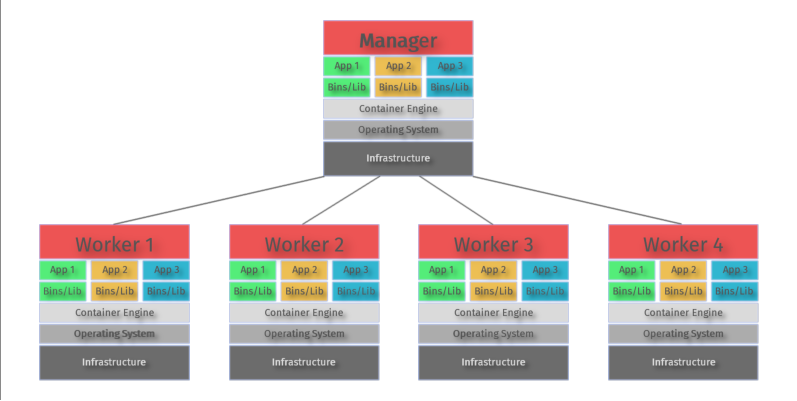
\includegraphics[width=1\textwidth]{img/cof}
    \caption{Darstellung eines Container Orchestration Frameworks \cite{Hick2019}}
    \label{fig:cof}
\end{figure}

\subsubsection{Kubernetes Control Plane} \label{subsec:control-plane}

Kubernetes ist ein von Google entwickeltes Container Orchestration Framework.
Für die Cloud-Native Entwicklung~\footnote{Cloud-Native Entwicklung: Entwicklung hoch skalierbarer- und verfügbarer Anwendungen unter der Annahme, Infrastruktur sei fast fehlerfrei\cite{8125550}.} eignet es sich besonders gut als Abstraktionsschicht zwischen Infrastruktur- und Anwendungsebene für eine einfachere, hardwareunabhängige Bereitstellung von Anwendungen, welche hochverfügbar oder skalierbar sein sollen.
Ein wesentlicher Bestandteil von Kubernetes ist die Control Plane, welche die zentrale Steuerung des Clusters zur Aufgabe hat.
Die Control Plane besteht aus mehreren Komponenten, welche je nach Anwendungsfall für einen hochverfügbaren Zugriff bereitgestellt werden können.
In jedem Fall besteht die Control Plane aus folgenden Komponenten:
\begin{itemize}
    \item \textbf{API Server:} Über den API Server erfolgt die Kommunikation mit Kubernetes und der Control Plane.
    Jede Interaktion mit einer Kubernetes Ressource lässt sich auf einen zugrunde liegenden Schnittstellenaufruf an den API Server zurückführen.
    \item \textbf{Controller Manager:} Eine Sammlung verschiedenster Kontrollprozesse, welche nach dem Unix Principle \emph{Do One Thing and Do It Well}~\cite{gancarz2003linux} aufgeteilt sind.
    \item \textbf{etcd:} Eine Key-Value-Datenbank, welche als Datenschicht für das Cluster und dessen Zustand zur Verfügung steht.
    \item \textbf{Scheduler:} Der Scheduler übernimmt die Aufgabe, Pods auf freie Knoten zu verteilen~\cite{kubernetesscheduler}.
\end{itemize}

Ein Cluster besteht in der Regel aus einer Gruppe virtueller oder echter Maschinen (VMs).
Im Kubernetes Kontext wird eine VM meist Knoten bzw. Node genannt.
Auf jedem Knoten finden sich die folgenden Komponenten:

\begin{itemize}
    \item \textbf{Kubelet:} Das Kubelet stellt sicher, dass provisionierte Pods entsprechend ihrer Konfiguration laufen.
    \item \textbf{kube-proxy:} Stellt die Kommunikation der Kubernetes Komponenten miteinander sicher.
\end{itemize}
Zur weiteren Lektüre bietet die Linux Foundation eine ausgezeichnete Dokumentation welche sich mit der Kubernetes Control Plane beschäftigt~\cite{kubernetescomponents}.
\subsubsubsection{Pod}
Der Pod ist die kleinste kubernetesspezifische Einheit.
Er besteht aus einem oder mehreren Containern, welche konform zu den Standards der Open Container Initiative (OCI) sind.
Die unter Entwicklern am weitesten verbreitete Methode, Container zu bauen, ist mit Hilfe von Docker.
Docker Container bieten die technische Grundlage, auf der die Standards der OCI basieren~\cite{opencontainerinitiative}.
Der Pod fungiert als ein Wrapper um seine Container, um diese als eine Einheit zu behandeln und in das Kubernetes Ökosystem integrierbar zu machen.
Die Hauptaufgabe des Pods ist es, Informationen über Ressourcenverbrauch sowie den Gesundheitszustand des Stücks Software, welches in den Containern läuft, zu sammeln und der Control Plane bereitzustellen.
Wird ein Pod aktualisiert, so muss dieser neu gestartet werden, da es sich dabei um eine unveränderliche Einheit handelt~\cite{kubernetespods}.

\subsubsubsection{Deployment}
Mehrere Pods, welche die Konfiguration und bereitgestellten Container teilen, können in einem Deployment zusammengefasst werden.
Ein Deployment bietet die Möglichkeit, mehrere Pods des gleichen Typs zentral zu verwalten.
So wird durch diese Komponente eine Vielzahl für moderne Softwaretechnik relevanter Funktionen bereitgestellt~\cite{kubernetesdeployments}:

\begin{itemize}
    \item \textbf{Skalierbarkeit:} Die Anzahl der gleichzeitig laufenden Pods kann über ein Deployment definiert werden.
    So kann Hochverfügbarkeit durch einfache Konfiguration des Deployments umgesetzt werden.
    \item \textbf{Rolling Updates:} Liegt Software in einer neuen Version vor, so muss diese auch ausgerollt werden.
    Wie oben geschrieben, kann der Container in einem Pod nicht einfach ausgetauscht werden.
    Durch rolling Updates wird sichergestellt, dass die neue Softwareversion in neuen Pods bereitsteht, bevor Pods mit der alten Version heruntergefahren werden.
    \item \textbf{Rollbacks:} Wurde eine Version bereitgestellt, welche fehlerhaft ist, so kann über ein Deployment einfach die vorherige Version wiederhergestellt werden.
\end{itemize}~\cite{kubernetesdeployments}

\subsubsubsection{Service}
Um ein Deployment verfügbar zu machen, kann ein Service definiert werden.
Je nach Typ erfüllt ein Service unterschiedliche Funktionen.
Laut Dokumentation~\cite{kubernetesservices} existieren die folgenden:

\begin{itemize}
    \item \textbf{ClusterIP:} Der Service erhält eine IP-Adresse, welche nur innerhalb des Clusters erreichbar ist.
    \item \textbf{NodePort:} Erlaubt den externen Zugriff auf den Service über das entsprechende Protokoll und den Port.
    Ermöglicht zudem die eigene Implementierung eines Loadbalancing Verfahrens.
    \item \textbf{LoadBalancer:} Ist das Kubernetes Cluster über einen Cloud-Provider provisioniert, so wird in diesem Fall automatisch ein Loadbalancer für den Service erstellt, welcher auf diesen verweist.
    \item \textbf{ExternalName:} Erlaubt das direkte Mapping eines Domain Name System (DNS)~\footnote{DNS: Technologie zur Auflösung von Domain Namen durch Abbildung von Domains auf IP-Adressen} Names auf einen Service~\cite{kubernetesservices}.
\end{itemize}

\subsubsection{Custom Resource Definitions}
Jede Interaktion mit einem Kubernetes Cluster stellt einen API-Aufruf an den API-Server der Control Plane (siehe Absatz~\ref{subsec:control-plane}) dar.
Custom Resource Definitions (CRDs) ermöglichen es dem Verwalter eines Kubernetes Cluster, die Schnittstelle der Control Plane um eigene Ressourcen zu erweitern, welche dann über die typischen Kubernetes Definitionen bereitgestellt werden.
So kann zum Beispiel ein Zertifikatsmanager zur Absicherung von Webservern und Endpunkten im Cluster über Secure Sockets Layer (SSL)-Zertifikate installiert werden, welcher Zertifikate als eigene CRD in einem Cluster zur Verfügung stellt~\cite{certman}.

\newpage
